\documentclass[11pt]{article}
\usepackage[margin=1in]{geometry}
\usepackage{amsmath}
\usepackage{graphicx}
\usepackage{booktabs}
\usepackage{xcolor}
\usepackage{caption}
\usepackage[hidelinks]{hyperref}
\usepackage{enumitem}

\definecolor{cainiao}{HTML}{0571B0}
\graphicspath{{../figures/}}
\captionsetup{font=small,labelfont=bf}

\title{\vspace{-1.5em}\textbf{Cainiao is Fast --- But Not Everywhere}\\[0.2em]
\large When does Alibaba's logistics network stop delivering its speed advantage?}
\author{BUAD 345: Decision Analytics and Visualization \\ Final Project}
\date{Summer 2026}

\begin{document}
\maketitle
\vspace{-1.5em}

\noindent\textbf{Audience: Cainiao (Alibaba's logistics platform).}\quad
\textbf{Data:} Tmall order, logistics, and merchant records, Jan 1--Jul 31, 2017
(1{,}291{,}197 orders; 1{,}288{,}438 with a complete, valid fulfillment time).

%======================================================================
\section*{1. Motivation}
In Chinese e-commerce, delivery speed is a primary driver of customer
satisfaction and repeat purchase, and it is the metric on which logistics
platforms compete most visibly.\footnote{Replace with an assigned reference,
e.g. a Cainiao/Alizila press item or an operations-management study on
delivery speed and customer retention.} Cainiao's value proposition is that its
smart-routing platform makes fulfillment \emph{faster}. In our data Cainiao
handles \textbf{30.2\%} of all orders, so any systematic weakness in its speed
advantage is material to the platform.

%======================================================================
\section*{2. Main Idea}
We test one focused question: \emph{does Cainiao actually make order fulfillment
faster, and if so, is that advantage uniform?} Our outcome is total fulfillment
time, defined exactly as in the course materials:
\[
\text{totaltime} \;=\; \text{SIGNED timestamp} \;-\; \text{pay\_timestamp}
\quad(\text{hours}).
\]
We then dig \emph{hierarchically}: carrier size, then destination-city size,
then a segment-level decomposition of where the time is spent.

%======================================================================
\section*{3. Findings}

\paragraph{3.1 Overall, Cainiao is faster.}
Cainiao orders are fulfilled in \textbf{61.9 h} on average versus \textbf{71.0 h}
for non-Cainiao orders --- about \textbf{9.2 hours faster} (medians: 53.7 vs
66.3 h). The gap survives a fair-comparison control: restricting to orders with
\emph{no} promised-speed window (\texttt{promise = 0}) leaves it essentially
unchanged (62.5 vs 71.0 h). See Figure~\ref{fig:main}.

\begin{figure}[h]
\centering
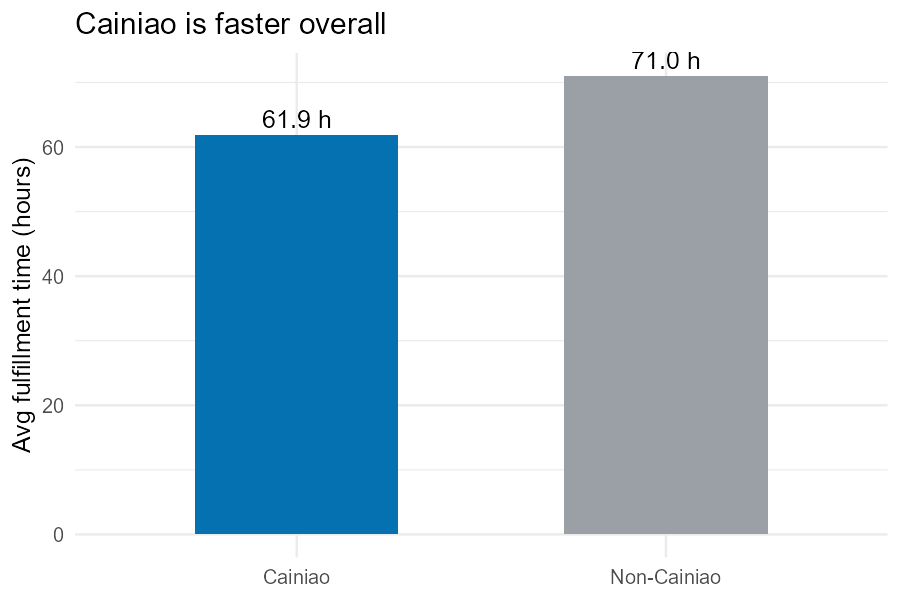
\includegraphics[width=0.52\textwidth]{fig1_main_effect.png}
\caption{Cainiao is faster overall.}
\label{fig:main}
\end{figure}

\paragraph{3.2 The advantage is uneven across carriers.}
Splitting by carrier size (``Large'' = a carrier handling $>$200{,}000 orders;
the two largest carriers cover the bulk of volume), Cainiao's edge is clearly
larger on large carriers than on small ones.

\paragraph{3.3 Punchline: big-city destinations on small carriers.}
Adding destination-city size (Big = the two largest destination cities) exposes
the real story. Cainiao saves 8--10.5 hours in three of the four cells --- but
in \textbf{big-city destinations handled by small carriers, Cainiao is actually
3.3 hours \emph{slower}} than non-Cainiao (Table~\ref{tab:cells},
Figure~\ref{fig:punch}).

\begin{table}[h]
\centering
\small
\caption{Average fulfillment time (hours) and Cainiao's advantage by cell.}
\label{tab:cells}
\begin{tabular}{llrrr}
\toprule
Destination & Carrier & Cainiao & Non-Cainiao & \textbf{Cainiao hours saved} \\
\midrule
Big city   & Large & 44.7 & 54.2 & \textbf{+9.5} \\
Big city   & Small & 52.4 & 49.1 & \textbf{\textcolor{red}{$-$3.3}} \\
Small city & Large & 61.7 & 72.2 & \textbf{+10.5} \\
Small city & Small & 67.1 & 75.2 & \textbf{+8.0} \\
\bottomrule
\end{tabular}
\end{table}

\begin{figure}[h]
\centering
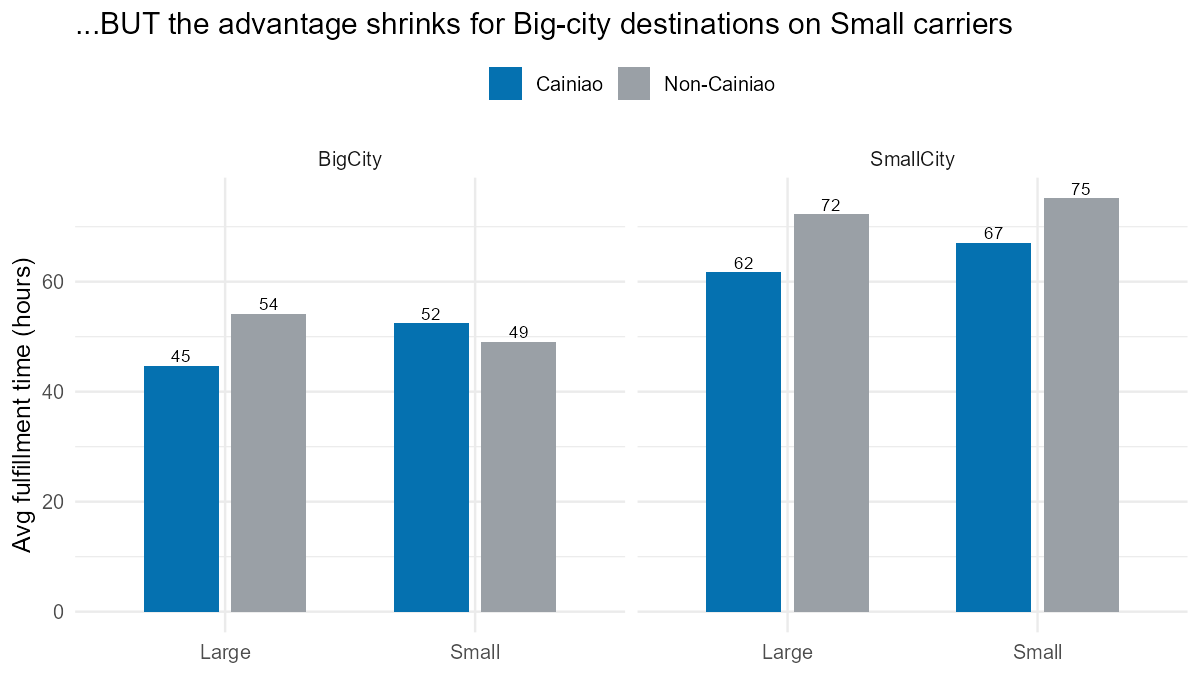
\includegraphics[width=0.85\textwidth]{fig2_punchline.png}
\caption{Cainiao's speed advantage nearly vanishes (and reverses) for big-city
destinations served by small carriers.}
\label{fig:punch}
\end{figure}

\paragraph{Customer reviews echo it.} The same cell is Cainiao's weakest on
logistics review score (4.764, its lowest of any cell, versus non-Cainiao's
4.860, the highest), so customers feel the slowdown too
(Figure~\ref{fig:review}).

%======================================================================
\section*{4. Mechanism: where does the time go?}
Decomposing fulfillment time into pre-delivery (order $\to$ pickup), line-haul
(between-facility transit), and last-mile (final station $\to$ buyer) shows the
gap lives in \textbf{line-haul, not the last mile}. Last-mile is small and
similar across all groups (roughly 4--6 h). Cainiao's usual edge comes from much
faster line-haul (e.g.\ 38.4 h vs 47.8 h on small-city/large-carrier orders) ---
but in the punchline cell that line-haul advantage disappears (27.0 h vs 26.9 h,
essentially tied). See Figure~\ref{fig:seg}.

\begin{figure}[h]
\centering
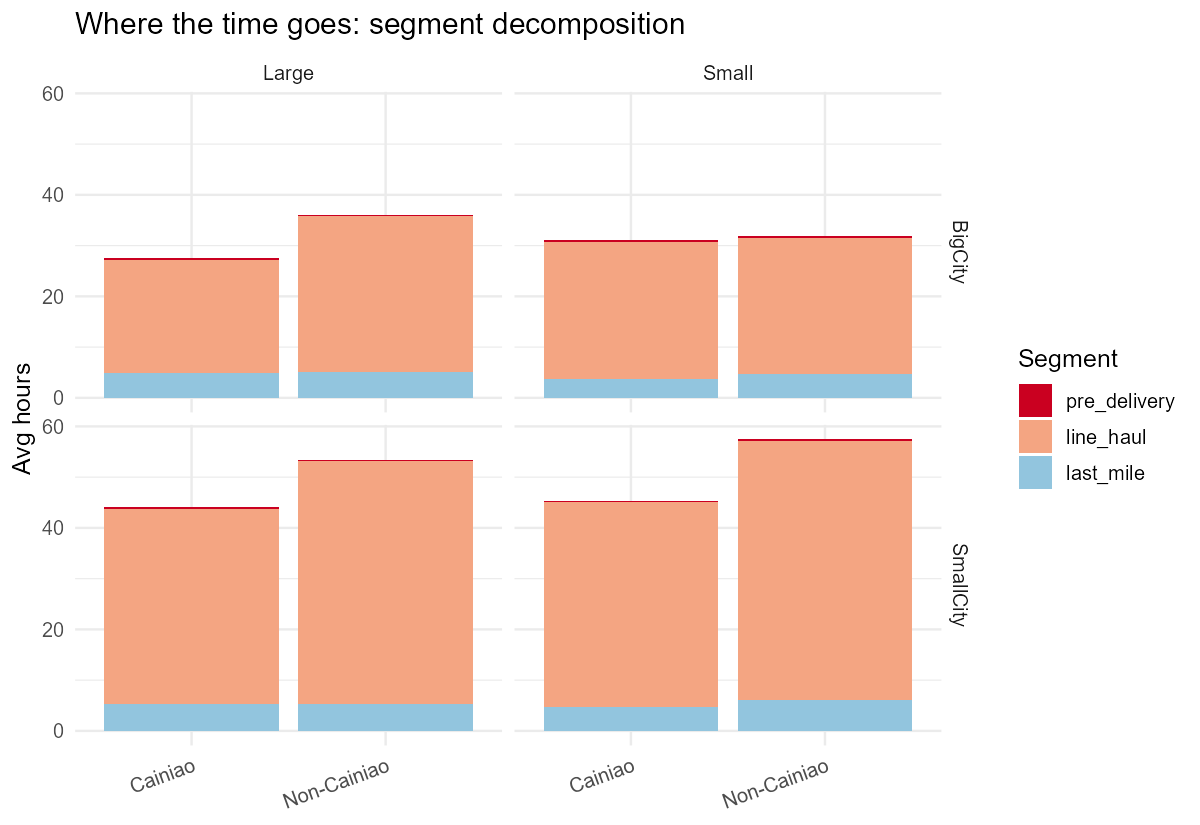
\includegraphics[width=0.8\textwidth]{fig3_segments.png}
\caption{Segment decomposition. The between-facility line-haul leg dominates and
is where Cainiao normally wins; that win evaporates for big-city/small-carrier
orders. (Segment means are computed over orders with complete milestones and are
not strictly additive to the totals in Table~\ref{tab:cells}.)}
\label{fig:seg}
\end{figure}

\begin{figure}[h]
\centering
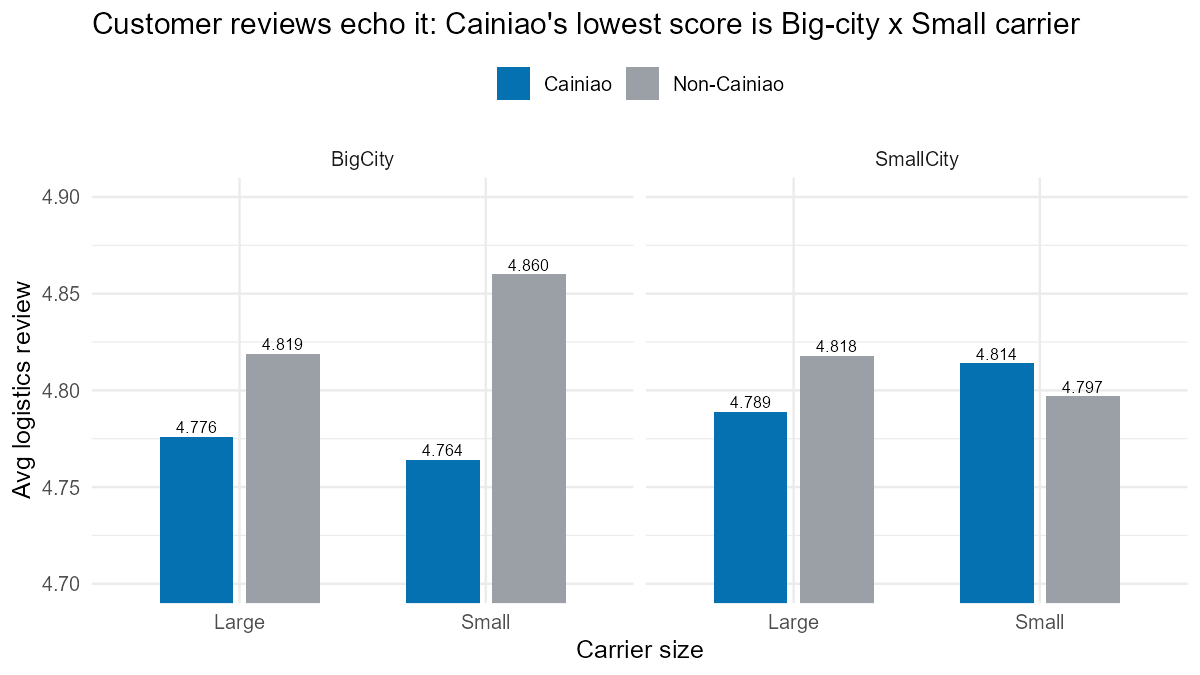
\includegraphics[width=0.8\textwidth]{fig4_review.png}
\caption{Customer reviews mirror the speed punchline.}
\label{fig:review}
\end{figure}

\paragraph{An honest non-result.} A natural hypothesis --- that small carriers
make more consolidation stops --- is \emph{not} supported: small carriers pass
through slightly \emph{fewer} cities on average (about 2.9--3.1) than large ones
(3.4--3.7). So the penalty is per-leg transit/dwell time, not a larger number of
hops.

%======================================================================
\section*{5. Potential Reasons}
Two domain explanations are consistent with the pattern. First, big cities
concentrate volume and inter-city trunk lines; large carriers run dedicated,
high-frequency line-haul into them, while small carriers must wait to consolidate
loads, adding transit/dwell time precisely on the high-expectation big-city
lanes.\footnote{Replace with an assigned reference on Chinese logistics
infrastructure / carrier line-haul economics.} Second, small carriers likely
lack the capacity to execute Cainiao's smart-routing recommendations as
designed, so the platform's optimization does not translate into time saved for
them.\footnote{Replace with an assigned reference on routing-algorithm
performance under heterogeneous carrier capability.}

%======================================================================
\section*{6. Practical Implications (So What?)}
For Cainiao:
\begin{enumerate}[leftmargin=1.4em,itemsep=2pt]
  \item \textbf{Deepen ties with large carriers} on big-city lanes for reliable
  speed --- while monitoring the concentration risk this creates.
  \item \textbf{Make smart-routing carrier-capability-aware} (size, coverage,
  experience) so small carriers are not assigned routes they cannot execute
  efficiently.
  \item \textbf{Pilot big-city consolidation / pickup lockers for small-carrier
  shipments} to attack the line-haul and pickup penalty where it actually
  occurs.\footnote{Replace with an assigned reference on pickup-point / locker
  effects on last-mile and consolidation efficiency.}
\end{enumerate}

%======================================================================
\section*{7. Limitations \& Causality}
This is observational data: assignment to Cainiao is not random, so differences
reflect association, not proven causation (e.g.\ merchants choosing Cainiao may
differ systematically). Milestone records are missing for some orders in this
real-world feed, so segment means use slightly different subsets than the totals.
The big-city flag is a coarse two-city proxy. These caveats temper the
magnitudes but not the qualitative punchline, which is large and consistent
across time, review scores, and segments.

%======================================================================
\section*{Two-Sentence Summary}
\textbf{(1)} Cainiao significantly shortens order fulfillment time across the
marketplace (about 9 hours on average). \textbf{(2)} But that advantage largely
disappears --- and even reverses --- for big-city destinations served by small
carriers, with the bottleneck in between-facility line-haul rather than the last
mile.

\end{document}
